\question{Отрицательная температура. Инверсная населенность энергетических 
уровней.}

Рассмотрим двухуровневую модель в состоянии термодинамического равновесия.
\begin{figure}[h!]
    \center
    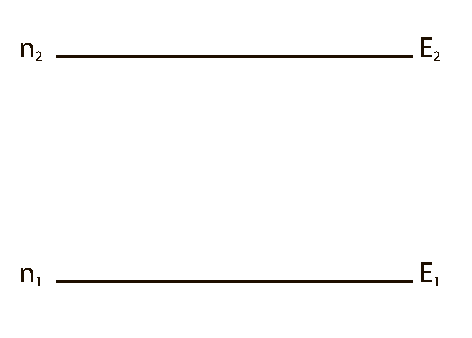
\includegraphics[width=.4\textwidth]{09_01} \hspace{1em}
    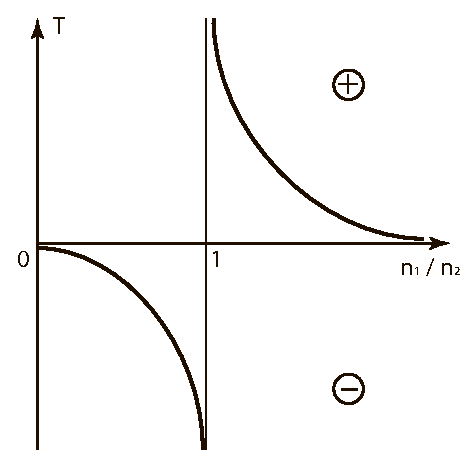
\includegraphics[width=.3\textwidth]{09_02} \\
    \parbox{.4\textwidth}{\caption{Двухуровневая система}} \hspace{1em}
    \parbox{.4\textwidth}{\caption{Зависимость \( T(n_1 / n_2) \)}}
\end{figure}

Населенность уровней подчиняется распределению Больцмана:
\[
    n_1 = n_0 \cdot \exp\left( -\frac{E_1}{kT} \right), \quad
    n_2 = n_0 \cdot \exp\left( -\frac{E_2}{kT} \right).
\]

Выразим температуру через населенности уровней:
\[
	\frac{n_2}{n_1} = \exp\left( -\frac{E_2-E_1}{kT} \right) 
    \quad \Rightarrow \quad
    \ln\frac{n_2}{n_1} = -\frac{E_2-E_1}{kT}
    \quad \Rightarrow \quad 
    T = \frac{E_2-E_1}{k\ln\cfrac{n_1}{n_2}}
\]

Возможны три случая:\\
1) \( n_1 / n_2 > 1 \Rightarrow T > 0 \) \\
2) \( n_1 / n_2 = 1 \Rightarrow T = \infty \) \\
3) \( n_1 / n_2 < 1 \Rightarrow T < 0 \)

Таким образом при изменении температуры от \( T = +0 \) до \( T = -0 \) через 
\( T = \pm\infty \) происходит переход частиц с нижнего уровня на верхний до 
полного опустошения нижнего уровня при полном заполнении верхнего уровня, то 
есть происходит переворот населённости. Другими словами -- инверсная 
населённость энергетических уровней.

\begin{figure}[h!]
	\center
	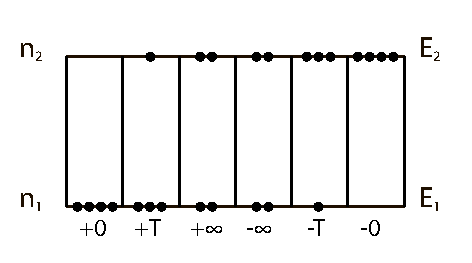
\includegraphics[width=.4\textwidth]{09_03}
\end{figure}

Особенности отрицательной температуры:
\begin{enumerate}
	\item состояние системы с отрицательной температурой имеет более высокую 
    	энергию, чем с положительной 
    \item отрицательную температуру можно получить лишь для конечного числа 
    	энергетических уровней. Это связано с тем, что для создания 
    	отрицательной температуры между парой уровней нужно затратить конечную 
    	энергию, а для бесконечного числа уровней -- бесконечное количество 
    	энергии.
\end{enumerate}
